\section{Simulações}

Simulações foram realizadas para testar os dispositivos projetados. Os testes avaliaram o funcionamento geral do circuito de acordo com as especificações do projeto, e também o funcionamento dos componentes APS e TIA.

Para a realização das simulações, é necessário se realizar uma estimativa da fotocorrente gerada dos fotodiodos. Como até o momento da simulação não havia a disponibilidade de uma amostra do fotodiodo, o autor fez uma estimativa conforme o trabalho de \cite{LidianeCampos}, apresentado na \autoref{tab_estcur}.

\begin{table}[htbp]
\caption{Estimativa de faixa de fotocorrente gerada}
\label{tab_estcur}
\centering
\begin{tabular}{cc}
\toprule
& Corrente nA \\
\midrule \midrule
Mínimo & 0,1\\
\midrule
Máximo & 30\\
\bottomrule
\end{tabular}
\legend{Fonte: Produzido pelo autor baseado no trabalho \cite{LidianeCampos}}
\end{table}

\subsection{Máximo sinal DC do APS}
\label{DCAPS}

É avaliado qual é o sinal DC que o bloco APS apresenta sem ter nenhuma fotocorrente gerada, $T_{enable}$ desabilitado e $T_{reset}$ habilitado. Na situação $V_{cn}$ irá apresentar o valor de VDD, o que vai representar o máximo sinal possível em $V_{out}$. A corrente \textit{Iref} considerada foi de $500$ nA, fornecida pelo bloco \textit{current\_mirror\_nmos}. Uma carga de $100$ fF foi utilizada na saída do APS de forma a simular a conexão com  um transistor na saída. O valor obtido foi de $1,15813$ V para $V_{out}$.

\subsection{Máximo sinal DC do APS no APS\_digitalized}

É avaliado qual é o sinal DC que o bloco APS conectado a um comparador apresenta sem ter nenhuma fotocorrente gerada, $T_{enable}$ desabilitado e $T_{reset}$ habilitado. Na situação $V_{cn}$ irá apresentar o valor de VDD, o que vai representar o máximo sinal possível em $V_{out}$. A corrente \textit{Iref} utilizada para a simulação foi de $500$ nA, fornecida pelo bloco \textit{current\_mirror\_nmos}. Uma carga de $100$ fF foi utilizada na saída do APS de forma a simular outras capacitâncias que podem aparecer no nó. O valor obtido foi de $1,15813$ V para $V_{out}$, equivalente ao apresentado na \autoref{DCAPS}.

\subsection{Máximo sinal DC do APS no APS\_digitalized}

É avaliado qual é o sinal DC que o bloco APS conectado a um comparador apresenta sem ter nenhuma fotocorrente gerada, $T_{enable}$ desabilitado e $T_{reset}$ habilitado. Na situação $V_{cn}$ irá apresentar o valor de VDD, o que vai representar o máximo sinal possível em $V_{out}$. A corrente \textit{Iref} utilizada para a simulação foi de $500$ nA, fornecida pelo bloco \textit{current\_mirror\_nmos}. Uma carga de $100$ fF foi utilizada na saída do APS de forma a simular outras capacitâncias que podem aparecer no nó. O valor obtido foi de $1,15813$ V para $V_{out}$, equivalente ao apresentado na \autoref{DCAPS}.

\subsection{Análise transiente do sinal de saída do APS}

É avaliado qual a resposta do APS com a presença de uma fotocorrente. Para a simulação, foi considerado o modelo apresentado na \autoref{fig_APS_cap}, do qual há uma fonte de corrente em paralelo a um diodo representando a fotogeração. A corrente \textit{Iref} considerada foi de $500$ nA, fornecida pelo bloco \textit{current\_mirror\_nmos}.

O Período de Reset é sempre definido para ter uma duração de $1$ us, de forma que esse valor precisa ser suficiente para que o sinal em $V_{cn}$ estabilize em VDD (como discutido na \autoref{secao_amostrando}). Dois valores para o Período de Integração foram considerados, como mostrado nas próximas subseções.

\subsection{Período de Integração igual a 121 $\mu$s}
\label{sub_sec121}

Nessa situação, foi considerado uma fotocorrente de 5 nA, que está dentro da faixa proposta pelo autor na \autoref{tab_estcur}. Os resultados obtidos são observados nos gráficos abaixo.

As figuras \ref{graf125} e \ref{graf1252} apresentam o comportamento esperado. Assim que RESET é desabilitado (vai para nível lógico '1'), Vout\_analogico passa a decair linearmente, como mostra \autoref{eq_modEletFotIl}\footnote{Note que aqui a tensão não foi completamente carregada por VDD, e por isso, ela inicia o ciclo de descarregamento em um ponto diferente de VDD.}. Quando Vout\_analogico atinge o valor de Vref, Vout\_digital vai do nível lógico '0' para '1', como descrito na \autoref{sec_apsdigitalized}.

\begin{figure}[htb]
 \centering
    \centering
    \caption{Tensão de saída analógica junto aos sinais de RESET e ENABLE para Período de Integração igual a 121 $\mu$s}
    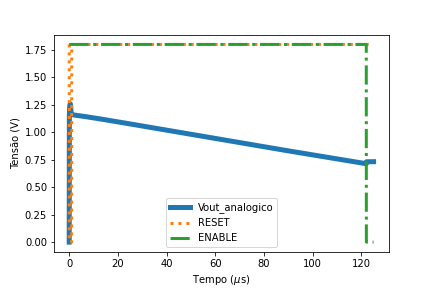
\includegraphics[scale=0.5]{Resultados/Graficos/reseteenable-tb_pixel125.png}
    \legend{Fonte: Produzido pelo autor}
    \legend{Nota: Vout\_analogico representa a tensão de saída analógica do APS}
    \label{graf125}
\end{figure}

\begin{figure}[htb]
 \centering
    \caption{Tensão de saída analógica e tensão de saída digital comparado à tensão de referência do Comparador Período de Integração igual a 121 $\mu$s} 
    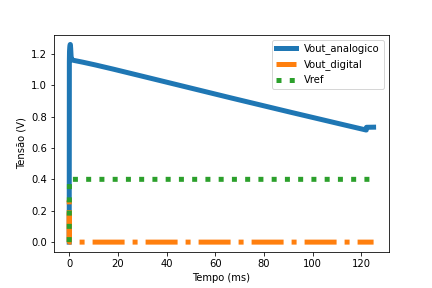
\includegraphics[scale=0.5]{Resultados/Graficos/analogicoedigital-tb_pixel125.png}
    \legend{Fonte: Produzido pelo autor}
    \legend{Nota: Vout\_digital representa a tensão de saída digital do APS\_digitalized}
    \label{graf1252}
\end{figure}

\subsection{Período de Integração igual a 247 $\mu$s}

Nessa situação, foi considerado uma fotocorrente de 2.5 nA, que está dentro da faixa proposta pelo autor na \autoref{tab_estcur}. Os resultados obtidos são observados nos gráficos abaixo.

As figuras \ref{graf247} e \ref{graf2472} apresentam mesmo comportamento daqueles apresentados na \autoref{sub_sec121}, como esperado.

\begin{figure}[htb]
 \centering
    \centering
    \caption{Tensão de saída analógica junto aos sinais de RESET e ENABLE para Período de Integração igual a 247 $\mu$s}
    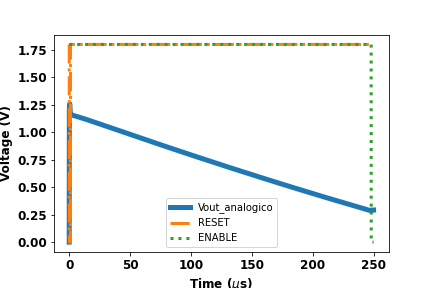
\includegraphics[scale=0.5]{Resultados/Graficos/reseteenable-tb_pixel250.png}
    \legend{Fonte: Produzido pelo autor}
    \legend{Nota: Vout\_analogico representa a tensão de saída analógica do APS}
    \label{graf247}
\end{figure}

\begin{figure}[htb]
 \centering
    \caption{Tensão de saída analógica e tensão de saída digital comparado à tensão de referência do Comparador Período de Integração igual a 247 $\mu$s} 
    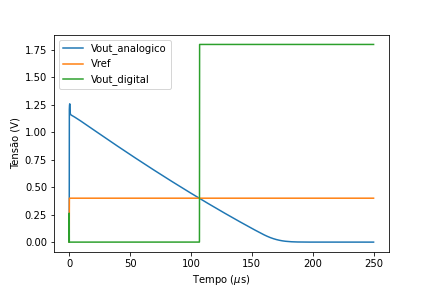
\includegraphics[scale=0.5]{Resultados/Graficos/analogicoedigital-tb_pixel250.png}
    \legend{Fonte: Produzido pelo autor}
    \legend{Nota: Vout\_digital representa a tensão de saída digital do APS\_digitalized}
    \label{graf2472}
\end{figure}

\subsection{Avaliação de ruído do APS\_digitalized}

Uma simulação para verificar a resposta ao ruído do APS\_digitalized foi realizado, de forma a verificar o impacto que um ruído pode ter ao sistema. O ruído pode aparecer por efeito térmico, cargas parasitas, ondas eletromagnéticas do ambiente entre diversos outras formas, tornando-o complexo de ser estimado. Uma simulação foi feita na previsão de ruídos de até 1 mV, mas o autor não garante que seja o valor exato de faixa possível de ruído.

\begin{figure}[htb]
 \centering
    \caption{Iterações de ruídos na faixa de 1 mV realizadas para simulação} 
    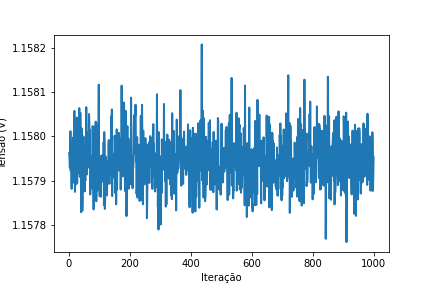
\includegraphics[scale=0.5]{Resultados/Graficos/ruido-Vout_noise.png}
    \legend{Fonte: Produzido pelo autor}
    \label{grafruido}
\end{figure}

A \autoref{grafruido} apresenta um gráfico com todas as iterações geradas para simulação, com sinal de tensão de ruído aplicado à saída do APS, que apresenta $T_{enable}$ desabilitado e $T_{reset}$ habilitado. Nessa situação, o autor do trabalho selecionou aleatoriamente 5 amostras do qual são demonstradas na , mas que são suficientes para as conclusões oferecidas.

\begin{figure}[htb]
 \centering
    \caption{Simulações de gráfico de ruído} 
    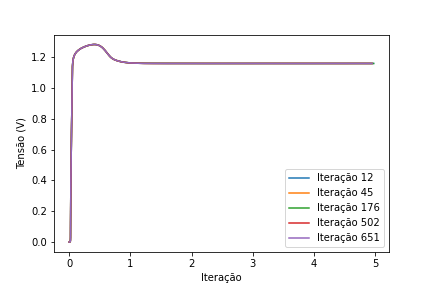
\includegraphics[scale=0.5]{Resultados/Graficos/tb_pixel_TRAN_NOISE.png}
    \legend{Fonte: Produzido pelo autor}
    \label{grafruido2}
\end{figure}

Como pode ser observado pela \autoref{grafruido2}, o ruído não impactou de forma visível a resposta do circuito, aparentando estarem todos visualmente sobre a mesma linha do gráfico.

\subsection{Análise transiente do sinal de saída do TIA}
\label{DCAPS}

Uma simulação do TIA foi realizada para averiguar se seu comportamento se apresenta adequado. Para as simulações foi utilizado Vref\_amp igual a 800 mV, e Vref\_comp igual a 1.3 V.

\begin{figure}[htb]
 \centering
    \caption{Corrente simulada de fotogeração} 
    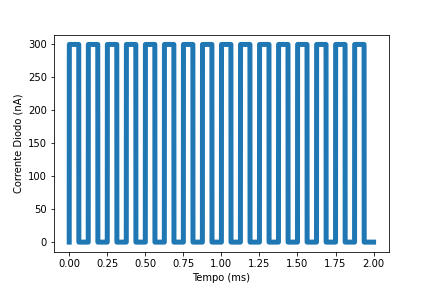
\includegraphics[scale=0.5]{Resultados/Graficos/Corrente Diodo-tb_clock.png}
    \legend{Fonte: Produzido pelo autor}
    \label{graf_tiasinal}
\end{figure}

\begin{figure}[htb]
 \centering
    \caption{Tensão de saída analógica do TIA} 
    \includegraphics[scale=0.5]{Resultados/Graficos/Tensao de Saída Analogica-tb_clock.png}
    \legend{Fonte: Produzido pelo autor}
    \label{graf_tiasinal2}
\end{figure}

\begin{figure}[htb]
 \centering
    \caption{Tensão de saída digital do TIA} 
    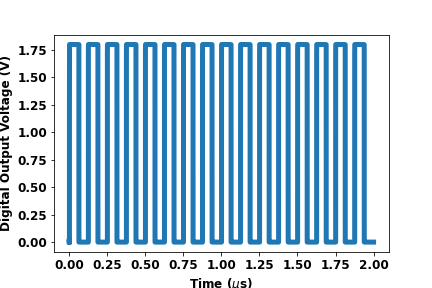
\includegraphics[scale=0.5]{Resultados/Graficos/Tensao de Saida Digital-tb_clock.png}
    \legend{Fonte: Produzido pelo autor}
    \label{graf_tiasinal3}
\end{figure}

O comportamento dos gráficos mostra um resultado adequado. Para uma fotocorrente de sinal quadrado, uma tensão quadrada de mesmo formato é gerada para a saída analógica e a digital.

